\documentclass[letterpaper]{article}

\usepackage[utf8]{inputenc}
\usepackage[english]{babel}
\usepackage{blindtext}
\usepackage{amsmath}
\usepackage{xfrac} % to have fraccions with diagonals using \sfrac
\usepackage{graphicx}
\usepackage{placeins} %stablish float barriers with \Floatbarrier
\usepackage{caption}
\usepackage{subcaption}
\usepackage{multirow}
\usepackage[hidelinks]{hyperref}
\usepackage{natbib}
\usepackage{booktabs}
\usepackage{siunitx} % required for alignment
\usepackage{tikz}
\sisetup{
			round-mode	= places, % Rounds numbers
			round-precision = 2 % to places
		}

\tikzset{
    treenode/.style = {shape=rectangle, rounded corners,
        draw, align=center,
        top color=white,
        bottom color=blue!20},
    root/.style     = {treenode, font=\normalsize,
        bottom color=blue!30},
    env/.style      = {treenode, font=\ttfamily\normalsize},
    dummy/.style    = {circle,draw}
}


\title{Establishing inventory policies through bootstrap estimations}
\author{Applicant: Luis Pérez - Advisor: Marco A. De Luna}
\date{November 2012}

\begin{document}
    
\maketitle
\pagenumbering{gobble}


\selectlanguage{english}
\bibliographystyle{apalike}

\begin{verse}
    This document, written on November 2020, serves as a summary of the research thesis conducted by the author in order to obtain the degree of \textit{Master in Science with a specialty in Quality Systems and Productivity}. With the absolute approval of the dissertation evaluation committee, this title was granted to the applicant by the Monterrey Institute of Technology and Higher Education --ITESM-- in November 2012.
    
\paragraph{}

\end{verse}



\begin{abstract}

One common assumption found in several inventory management models is that the lead time demand follows a normal  probability distribution. If such models are used in spite of the normality premise being false, the resultant policies might negatively impact the system performance by having excessive inventory or achieving a low customer service level. Both of these results are undesirable since in the case of the former the holding cost would rise, whereas in the latter the shortage cost would grow.
\paragraph{}
This research focuses on evaluating the effectiveness of a proposed distribution free algorithm that determines the inventory target level $(S)$ in a periodic review model $(S,T)$. The algorithm relies heavily on the statistical tool known as bootstrap although several additional techniques are involved too.
\paragraph{}
The data used for this investigation corresponds to the actual observed behavior of 31 items sold by an independent electrical and lighting retailer. Through Dynamic Simulation a benchmark between the resulting policies from both the traditional $(S,T)$ model and the proposed algorithm is performed; the corresponding performances are measured in terms of the ability to reach the desired customer service level along with the associated cost.
\paragraph{}
The study reveals that despite the fact that none of these approaches can guarantee that the desired service level will be achieved, the proposed algorithm has a higher chance of doing it. Moreover, the costs linked to the policies determined by the presented algorithm turned out to be lower in most cases.

\paragraph{}
keywords: \textit{Inventory policies,} $(S,T)$, \textit{bootstrap, distribution-free, dynamic simulation, retail distribution}


\end{abstract}

\section*{Introduction and background}
\paragraph{}
According to \citet*{chopra2007supply} successful supply chain management requires taking decisions regarding the flow of information, products and resources. Particularly in the planning phase, companies define the policies that rule their operations in the short term. Among them, the inventory policies stand out for their relevance.

\paragraph{}
Furthermore, the financial success of a company depends to a great extent on the adequacy of the inventory policies to satisfy the demand it faces. If the demand is not met sales will be lost. In the other hand, an excessive inventory leads to a waste of resources.

\paragraph{}
One of the most important models to manage inventories is the periodic review model, also known as $(S,T)$ model. It controls the inventory by issuing purchase orders --aka. PO-- at intervals with a predefined length of $T$. Once the interval has elapsed, the positional inventory reaches a given inventory target level $(S)$ by issuing a PO.

\paragraph{}
\citet*{waller2008review} point out that even though the adoption of the $(S,T)$ model is quite frequent, its study has been scarce. In their review, only few articles --\citet*{blumenfeld1984trade}, \citet*{hsu1991integrating}, \citet*{ballou2005expressing} and \citet*{sezen2006changes}-- use the periodic review system either as one of several inventory control policies or the only one. 

\paragraph{}
Unfortunately, a wide spread \textit{assumption} found in the relevant literature is that the lead time demand properly fits a normal probability distribution. In consequence, this assumption underlies in the "run of the mill" formulas generally used by professionals and coded into commercial ERP software packages. Obviously, if such formulas are used despite the lead time demand being non-normal, the resulting policies will most likely generate either lost sales or an inventory excess; both outcomes are undesirable since they negatively impact the financial performance of the company.

\subsection*{The periodic review model $(S,T)$}
\paragraph{}
In the $(S,T)$ model, the positional inventory, composed by the on-hand inventory and the in-transit inventory, is calculated at intervals with a fixed length, $T$. If the positional inventory turns out to be below its target level $(S)$, a purchase order for a quantity that covers up for the difference $(Q)$ is issued. 

\begin{align}
    I_\mathrm{positional}  &= I_\mathrm{on-hand} + I_\mathrm{in-transit} \\
    Q &= S - I_\mathrm{positional}
\end{align}

\paragraph{}
The common application of the $(S,T)$ model consists of determining the positional inventory target level --$S$-- given a previously defined review interval length $T$. The frequently used notation is shown in table \ref{tab:reg_ST_notation}.

\begin{table}[!h]
    \begin{center}
        \begin{tabular}{c|l}
            \toprule
            $D$ & Demand per time unit. \\
            $\sigma$ & Demand standard deviation per time unit.\\
            $\tau$ & Lead time; Assumed deterministic. \\
            $T$ & Revision period length. \\
            $S$ & Positional inventory target level. \\
            \bottomrule
        \end{tabular}
    \end{center}
    \caption{The $(S,T)$ model notation}
    \label{tab:reg_ST_notation}
\end{table}


\subsection*{The \textit{traditional} $(S,T)$ model}

\paragraph{}
As discussed, the \textit{traditional} model works with an stochastic revision and lead time demand (RLTD) which is \textit{assumed} to be normal. Furthermore, another quite simplistic approach of the traditional model is to treat the lead time as a deterministic variable. With this in consideration, a typical behavior of the on-hand inventory through time is illustrated on figure \ref{fig:trad_st_behavior}.

\begin{figure}[!h]
    \centering
        \includegraphics[width=0.8\textwidth]{./figs/ST_ideal_eng_600x300px.png}
    \caption{Example of the inventory behavior\linebreak in a traditional $(S,T)$ model}
    \label{fig:trad_st_behavior}
\end{figure}

\paragraph{}
For the traditional model the notation consists of what was stated in table \ref{tab:reg_ST_notation} in addition to the content of table \ref{tab:trad_ST_notation}.

\begin{table}[!h]
    \begin{center}
        \begin{tabular}{c|l}
            \toprule
            $\overline{D}$ & Average demand per time unit. \\
            $\overline{D}_{T+\tau}$ & Average revision and lead time demand.\\
            $\sigma_{T+\tau}$ & Revision and lead time demand std. deviation. \\
            \multirow{2}{*}{$z_{(1-\alpha)}$} & 
            \begin{minipage}[t]{0.8\columnwidth}
                $1-\alpha$ percentile value of the  standard normal distribution probability that matches the desired in-stock probability, i.e., target service level.	
            \end{minipage} \\
            \bottomrule
        \end{tabular}
    \end{center}
    \caption{Complimentary notation for the traditional $(S,T)$ model}
    \label{tab:trad_ST_notation}
\end{table}

\paragraph{}
The mean and the standard deviation of the RLTD are given by equations \ref{eq:traditional_RLTD_mean} and \ref{eq:traditional_RLTD_stdev} respectively.

\begin{align}
    \overline{D}_{T+\tau} &= \overline{D}(T+\tau) \label{eq:traditional_RLTD_mean}\\
    \sigma_{T+\tau} &= \sigma\sqrt{T+\tau} \label{eq:traditional_RLTD_stdev}
\end{align}

\paragraph{}
Due to the fact that the $\mathrm{RLTD}$ is treated as normal, the positional inventory target level $(S)$ is defined as follows:

\begin{equation}\label{eq:traditional_RLTD_S}
    S = \overline{D}_{T+\tau} + z_{(1-\alpha)}\sigma_{T+\tau}
\end{equation}

\paragraph{}
Figure \ref{fig:RLTD_distribution_normality} shows an example of a KDE plot of the RLTD along with the $S$ estimation location over the $D_{T+\tau}$ axis for this scenario. In order to ease the grasp of the algorithm that will be presented next, it is extremely important to realize that as shown in this figure, the positional inventory target level $S$ is nothing else than the $1-\alpha$ percentile value of the RLTD. In this context, $1-\alpha$ represents the targeted in-stock probability, i.e. desired service level.

\begin{figure}[!hbt]
    \centering
    \includegraphics[width=0.8\textwidth]{./figs/RLTD_distribution_normality.png}
    \caption{KDE plot of the $RLTD$ in the traditional $(S,T)$ model}
    \label{fig:RLTD_distribution_normality}
\end{figure}


\FloatBarrier

\subsection*{More objections to the traditional $(S,T)$ model}
\paragraph{}
Besides the main objection to the assumption of normality there are a couple more aspects of the traditional $(S,T)$ model that are highly questionable by those who have had "field" experience in determining inventory policies.

\begin{itemize}
	\item[•]$\tau$ treated as deterministic. In the day-to-day reality lead times can vary greatly; delays from the supplier take place up to the point of $\tau$ being several times higher than $T$ making the behavior of the system something similar to what is shown in figure \ref{fig:real_st_behavior}.
	\item[•]Regardless of we consider $\tau<T$ or  $\tau>T$, undoubtedly $\tau$ and $T$ overlap each other. In light of this, the logic behind equation \ref{eq:traditional_RLTD_S} is quite dubious. Therefore to emphasize this disagreement, from this point $D_\omega$ will be used to represent the demand that takes place during the overlapped lead time and revision period, replacing ${D}_{T+\tau}$.
\end{itemize}

\begin{figure}[!hbt]
    \centering
    \includegraphics[width=0.8\textwidth]{./figs/ST_reality_eng_600x300px.png}
    \caption{Example of the inventory behavior \linebreak in a realistic $(S,T)$ model}
    \label{fig:real_st_behavior}
\end{figure}

\FloatBarrier

\section*{Overview of the relevant statistical tools}
\paragraph{}
The algorithm to be presented in the next section relies in several statistical tools which quick revisions are deemed as pertinent in order to ease the reading of this document. Namely:

\begin{itemize}
    \item The bootstrap - \cite{efron1979bootstrap}.
    \item The jackknife - \cite{quenouille1949approximate}.
    \item Asymmetry significance testing - \cite{tabachnick2000using}.
    \item Bootstrap $\mathrm{BC}_a$ confidence intervals - \cite{efron1994introduction}.
    \item Data transformation for robust bootstrap estimation - \cite{singh1998breakdown}.
\end{itemize}

\FloatBarrier

\subsection*{The bootstrap}
\paragraph{}
The bootstrap methods --\cite{efron1979bootstrap}-- depend on the notion of a \textit{bootstrap sample}. Let $\hat{F}$ be an empirical distribution of the random variable $X$, putting a probability of $1/n$ on each of the observed values $x_i$, $i=1,2,\cdots,n$. A bootstrap sample is defined to be a random sample of size $n$ drawn from $\hat{F}$, say 

\begin{align}
    \hat{F}\rightarrow[x_1,x_2,&\cdots,x_n] \\
    \vec{x}_b=[x_{1_b},x_{2_b},&\cdots,x_{n_b}]
\end{align}

\paragraph{}
The $b$ sub index indicates that $\vec{x}_b$ is not the actual data set $\vec{x}$, but rather a randomized, or re-sampled, version of it. In other words, the bootstrap data points are a random sample of size $n$ \textit{with replacement} from the original observed values $x_1,x_2,\cdots,x_n$. Thus we might have $x_{1_b}=x_7,x_{2_b}=x_3,\cdots,x_{n_b}=x_1$. The bootstrap data set $[x_{1_b},x_{2_b},\cdots,x_{n_b}]$ consists of members of the original data set $[x_1,x_2,\cdots,x_n]$ some appearing zero times, some appearing twice, etc.

\paragraph{}
Corresponding to a bootstrap sample $\vec{x}$, a \textit{bootstrap replica} is defined as:

\begin{equation}
    \hat{\theta}_b=s(\vec{x}_b)
\end{equation}

\paragraph{}
Where $\hat{\theta}_b$ is the results of applying any given function $s$ to the data set $[x_{1_b},x_{2_b},\cdots,x_{n_b}]$ as if it was a applied to a \textit{regular} sample of the random variable $X$, in order to estimate a parameter of interest $\theta$. The notation $\hat{\theta}$ indicates that we are talking about an \textit{estimation} of the parameter $\theta$, not its true value, whereas $\hat{\theta}_b$ is used to represent an estimation of the parameter of interest calculated from a bootstrap sample.

\paragraph{}
A bootstrap algorithm works by drawing many independent samples, and evaluating the corresponding bootstrap replicas which results are stored in a vector e.g. $\vec{\hat{\theta}}_b$. From there a punctual estimation of the parameter of interest as well as the standard error --given by the sample standard deviation-- can be calculated as:

\begin{align}
        \hat{\theta}_{b(\cdot)}&=\sum_{\hat{\theta}_b\in\vec{\hat{\theta}}_b}\hat{\theta}_b\cdot\left(1/\#\vec{\hat{\theta}}_b\right) \\
        \hat{\mathrm{se}}_{\hat{\theta}_b}&=\left[\sum_{\hat{\theta}_b\in\vec{\hat{\theta}}_b}\left(\hat{\theta}_b-\hat{\theta}_{b(\cdot)}\right)^2/\left(\#\vec{\hat{\theta}}_b-1\right)\right]^{1/2}
\end{align}

\paragraph{}
Let $B$ represent the number of bootstrap replicas. As $B\rightarrow\infty$, $\hat{\mathrm{se}}_{\hat{\theta}_b}$ approaches $\hat{\mathrm{se}}_{\hat{\theta}_{\hat{F}}}$. In consequence, the number of bootstrap replicas --$B$--  that are enough to properly estimate the standard error is between 25 to 200.

\FloatBarrier

\subsection*{The jackknife}
\paragraph{}
The jackknife is a technique for estimating both the bias and the standard error of an estimate. It precedes the bootstrap and bears close similarities to it. Suppose we have a sample $\vec{x}=[x_{1},x_{2},\cdots,x_{n}]$ . The jackknife focuses on re-sampling the original data set \textit{leaving out one observation at a time}:

\begin{equation}
    \vec{x}_j=[x_1,x_2,\cdots,x_{i-1},x_{i+1},\cdots,x_n]
\end{equation}

\paragraph{}
for $i=1,2,\cdots,n$, called jackknife samples. The $i$th jackknife sample consists of the original data set with the $i$th observation removed. Let 
\begin{equation}
    \hat{\theta}_{j(i)}=s(\vec{x}_{j(i)})
\end{equation}
\paragraph{}
be the $i$th jackknife replication of $\hat{\theta}$. The jackknife estimate of bias is defined by
\begin{equation}
    \hat{\mathrm{bias}}_\mathrm{jack}=(n-1)(\hat{\theta}_{j(\cdot)}-\hat{\theta})
\end{equation}
\paragraph{}
where
\begin{equation}
    \hat{\theta}_{j(\cdot)}=\sum_{i=1}^{n}\hat{\theta}_{j(i)}/n
\end{equation}

\FloatBarrier

\subsection*{Bootstrap $\mathrm{BC}_a$ confidence intervals}

\paragraph{}
\cite{efron1994introduction} remark that one of the principal goals of the bootstrap is to produce good confidence intervals. In this context, "good" means that the bootstrap intervals should closely match exact confidence intervals in those special situations where statistical theory yields an exact answer, and should give dependably accurate coverage probabilities in all situations. 

\paragraph{}
Among the several methods available to construct confidence intervals by making use of the bootstrap, $\mathrm{BC}_a$ --\textit{bias corrected and accelerated} -- intervals are the ones that come closest to the before mentioned criteria of goodness; The downside of the $\mathrm{BC}_a$ confidence intervals is that they are also the most computationally expensive to produce as they involve the use of the jackknife.

\paragraph{}
The bias correction coefficient, $z_0$, is calculated by

\begin{equation}
    \hat{z}_0=\Phi^{-1}\left[\frac{\#\left(\left\{\hat{\theta}_b\in\vec{\hat{\theta}}_b\right\}<\hat{\theta}\right)}{\#\vec{\hat{\theta}}_b}\right]
\end{equation}
\paragraph{}
where $\Phi^{-1}$ is the standard normal inverse cumulative distribution function. For example $\Phi^{-1}(0.95)=1.645$.

\paragraph{}
The acceleration coefficient $\hat{a}$ refers to the rate of change of the standard error of $\hat{\theta}$ with respect to the true parameter value of $\theta$, \textit{measured on a normalized scale}. It is calculated with the formula:
\begin{equation}
    \hat{a}=\frac{\sum_{i=1}^{n}\left(\hat{\theta}_{j(\cdot)}-\hat{\theta}_{j(i)}\right)^3}{6\left\{\sum_{i=1}^{n}\left(\hat{\theta}_{j(\cdot)}-\hat{\theta}_{j(i)}\right)^2\right\}^{3/2}}
\end{equation}

\paragraph{}
Let $\alpha$ represent the type I error probability. The $\mathrm{BC}_a$ interval of intended coverage $1-2\alpha$ is given by
\begin{equation}
    \mathrm{BC}_a: \left[\hat{\theta}_\mathrm{bLo},\hat{\theta}_\mathrm{bUp}\right]= \left[\mathrm{percentile}_{\alpha_1}\left(\vec{\hat{\theta}}_{b}\right),\mathrm{percentile}_{\alpha_2}\left(\vec{\hat{\theta}}_{b}\right)\right]
\end{equation}
\paragraph{}
where
\begin{align}
     \alpha_1&=\Phi\left[\hat{z}_0+\frac{\hat{z}_0+z_{(\alpha)}}{1-\hat{a}\left(\hat{z}_0+z_{(\alpha)}\right)}\right] \\
     \alpha_2&=\Phi\left[\hat{z}_0+\frac{\hat{z}_0+z_{(1-\alpha)}}{1-\hat{a}\left(\hat{z}_0+z_{(1-\alpha)}\right)}\right]
\end{align}
\paragraph{}
Here $\Phi$ represents the standard normal cumulative distribution function whereas $z_{(a)}$ is the $100\alpha$th percentile value of the standard normal probability distribution. For example $z_{(0.95)}=1.645$ and $\Phi(1.645)=0.95$.

\FloatBarrier

\subsection*{Asymmetry significance testing}
\paragraph{}
When a random variable follows a normal probability distribution its asymmetry and kurtosis values are equal to zero. According to \cite{tabachnick2000using} there are asymmetry significance tests that try the actual value against the null hypothesis of zero. This is

\begin{align}
    H_0: S&=0 \\
    H_1: S&\ne0
\end{align}

\paragraph{}
The standard error of the asymmetry can be estimated by

\begin{equation}
    \hat{\mathrm{se}}_S=\sqrt{6/n}
\end{equation}

\paragraph{}
where $n$ is the quantity of observations in the sample. The asymmetry coefficient calculated from the sample --$S$-- is then compared to the value of 0 proper of a standard normal distribution. This will enable us to calculate $z$ by using

\begin{equation}
    z=\frac{S-0}{\hat{\mathrm{se}}_S}
\end{equation}

\paragraph{}
which in turn will allow us to determine the $p\mathrm{-value}$ required to perform the hypothesis test as

\begin{equation}
    p\mathrm{-value}=2\left[1-\Phi(z)\right]
\end{equation}

\paragraph{}
where as usual, $\Phi$ represents the cumulative function of the standard normal distribution. If with the $\alpha$ significance level $H_0$ is rejected, i.e. $p\mathrm{-value}<\alpha$, we could conclude that statistically the observed $S$ coefficient is different than zero and therefore the asymmetry in the sample is significant.

\FloatBarrier

\subsection*{Data transformation for robust bootstrap estimation}
\paragraph{}
\cite{singh1998breakdown} state that in the robust bootstrap estimation, extreme values have little to no influence in the obtained estimator. In consequence, some of the values at the extremes of $\vec{x}_s$ --the \textit{sorted} version of the sample data set $\vec{x}$-- could be modified to further increase the robustness of bootstrap percentiles.

\paragraph{}
In a data set $\vec{x}_s$ with $n$ observations the integer $l$ is calculated by

\begin{equation}
    l=\left\lfloor{n\beta}\right\rfloor
\end{equation} 


\paragraph{}
where the coefficient $\beta$, with a value between 0 and $\sfrac{1}{2}$, represents the $\beta\mathrm{-th}$ fraction of the data that will be transformed according to the logic of figure \ref{fig:data_transf}.\linebreak

\begin{figure}[h!]
    \begin{center}
        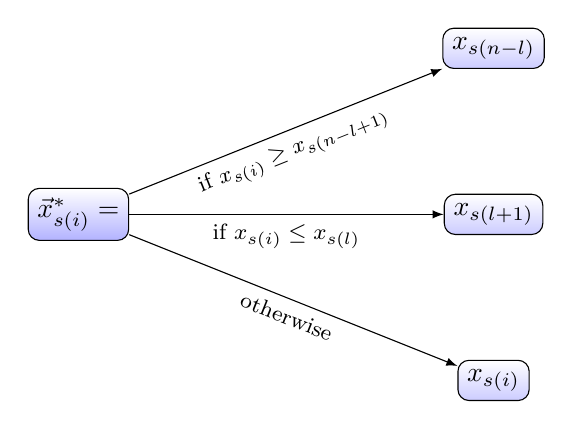
\begin{tikzpicture}
            [
            grow                    = right,
            sibling distance        = 6em,
            level distance          = 15em,
            edge from parent/.style = {draw, -latex},
            every node/.style       = {font=\footnotesize},
            sloped
            ]
            \node[root] (root) {$\vec{x}^*_{s(i)}=$}
                child {node[env]{$x_{s(i)}$}
                    edge from parent node [below] {otherwise}}
                child {node[env]{$x_{s(l+1)}$}
                    edge from parent node [below] {if $x_{s(i)}\le{x_{s(l)}}$}}
                child {node[env]{$x_{s(n-l)}$}
                    edge from parent node [below] {if $x_{s(i)}\ge{x_{s(n-l+1)}}$}}            
            ;
    \end{tikzpicture}
\caption{\textit{winsorization} data transformation logic\linebreak\cite{singh1998breakdown}}
\label{fig:data_transf}
    \end{center}
\end{figure}

\paragraph{}
Here $\vec{x}^*_{s(i)}$ represents the transformed --\textit{winsorized}-- data set from which the bootstrap samples will be generated. \cite{singh1998breakdown} sustain that despite the fact any $\beta<\sfrac{1}{2}$ value is theoretically valid, in practice $\beta$ should be set significantly below that value, e.g. $\beta\le\sfrac{1}{4}$.

\FloatBarrier


\section*{A new proposal for the estimation of $S$}
\subsection*{Assumptions and required information}
\paragraph{}
The algorithm takes a more realistic approach compared to the traditional model by assuming that the available information about the RLTD, $D_\omega$, is in fact accessible through \textit{real-life observations} of two independent random variables:

\begin{itemize}
	\item[•]Demand per time unit, $D$.
	\item[•]Lead time, $\tau$.
\end{itemize}

\paragraph{}
Additionally, the following parameters must be previously defined:
\begin{itemize}
	\item[•]Review interval length, $T$.
	\item[•]Desired service level, $1-\alpha$, i.e. the in-stock probability.
\end{itemize}

\paragraph{}
During the research the hardest obstacle to overcome was to obtain the \textit{actual demand} information for the studied items. The reason for this is that the vast majority of the companies do keep a record of their sales figures, but in the case of the demand its data is rarely available. 

\paragraph{}
It is worth recalling that $1-\alpha$ corresponds to the desired in-stock probability and that consequently the $1-\alpha$ percentile of $D_\omega$ determines the $S$ value in a periodic review system. Accordingly, $\theta$ will be used to represent our parameter of interest i.e. $\theta=\mathrm{percentile}_{1-\alpha}(D_\omega)$.


\paragraph{}
The pseudo code for the algorithm that estimates the positional inventory target level $(S)$, is divided across 4 main blocks:

\begin{enumerate}
	\item Data asymmetry testing and transformation.
	\item Generation of $D_\omega$ sample values.
	\item Evaluation of $\hat{\theta}$ bootstrap replicas.
	\item Construction of $\mathrm{BC}_a$ confidence intervals for $\theta$.
\end{enumerate}

\FloatBarrier


\subsection*{Algorithm Block 1: data asymmetry testing and transformation}
\paragraph{}
A common problem while working with demand and lead time data is the presence of extreme values. Such observations might cause that the empirical distribution of $D_\omega$ to end up with a long right tail; As a result its estimated  $1-\alpha$ percentile value would be significantly higher, leading to a bigger positional inventory target level and thus a larger holding cost.

\paragraph{}
Since the presence of extreme values would most likely result in a higher asymmetry, a hypothesis test to evaluate whether or not the asymmetry turns out to be significant is performed as proposed by  \cite{tabachnick2000using}. In the case that the null hypothesis is rejected, i.e. $H_0: S=0$, a portion of the observations at both ends will be transformed using the method suggested by \cite{singh1998breakdown}.

\paragraph{}
Another situation that could arise when working with real data of $D$ is the presence of zero --no demand-- or negative values --returns surpassing the demand-- among the observations. \cite{johansen2000r} make a justification to drop the negative values; As for the zero values, it was decided to also drop them in order to aim for a resulting higher service level.


\begin{enumerate}
	\item Create the vectors --1-D arrays--  $\vec{\tau}$ and $\vec{d}$ from the available $\tau$ and $D$ observations.
	\item Perform an asymmetry test on the $\vec{\tau}$ and $\vec{d}$ values.
	\begin{itemize} 
		\item[-] If $H_0$ is rejected, transform the data of the corresponding vector.
	\end{itemize}
	  
\end{enumerate}

\FloatBarrier

\subsection*{Algorithm Block 2: generation of $D_\omega$ sample values}
\paragraph{}
Up to this point, the available information of the $\mathrm{RLTD}$ is available on $\vec{\tau}$ and $\vec{d}$ values. By making use of the bootstrap, $\vec{\tau}$ and $\vec{d}$ observations will be mixed to generate $D_w$ sample values. 


\begin{enumerate}
	\setcounter{enumi}{2}
	\item Initialize $\vec{d}_{w}$ as an empty vector,
		\begin{equation}
			\vec{d}_w=\emptyset
		\end{equation}
	\item Determine the bootstrap sample size, $n$, that will be used as follows:
		\begin{equation}
			n =\left\lceil\frac{\#\vec{d}+\#\vec{\tau}}{2}\right\rceil
		\end{equation}
	\item While $\#\vec{d}_w<300$:
		\begin{enumerate}
			\item Generate a bootstrap sample of size $n$ from $\vec{\tau}$, $\vec{\tau}_b$
			\item Generate a vector of size $n$, $\vec{t}$ where $\forall{t}\in{\vec{t}}$, $t=T$
			\item $\vec{m}_b = \max({\vec{\tau}_b, \vec{t}})$
			\item Generate a bootstrap sample of size $n$ from $\vec{d}$, $\vec{d}_b$
			\item $\vec{d}_{w_b}=\vec{m}_b\odot{\vec{d}_b}$
			\item Add the values of $\vec{d}_{w_b}$ to $\vec{d}_{w}$
			\item $\vec{\tau}_b=\vec{m}_b=\vec{d}_b=\vec{d}_{w_b}=\emptyset$
		\end{enumerate}
\end{enumerate}

\paragraph{}
The condition established in the fifth step determines that the number of elements in $\vec{d}_w$ should be at least 300. This sample size for $D_w$ certainly seems reasonable if the rule of thumb $B=200$ set by \cite{efron1994introduction} to estimate standard errors is considered as a reference.

\FloatBarrier

\subsection*{Algorithm Block 3: evaluation of $\hat{\theta}$ bootstrap replicas}
\paragraph{}
Now that sample values of $D_\omega$ are available, the bootstrap will be used once again in order to make estimations of the parameter of interest $\theta$, which is the $1-\alpha$ percentile value of $D_\omega$.


\begin{enumerate}
	\setcounter{enumi}{5}
	\item Initialize $\vec{\hat{\theta}}_b$ as an empty vector,
		\begin{equation}
			\vec{\hat{\theta}}_b = \emptyset
		\end{equation}
	\item While $\#\vec{\hat{\theta}}_b<2000$:
		\begin{enumerate}
			\item Take a bootstrap sample from $\vec{d}_\omega$, $\vec{d}_{w_b}$
			\item Evaluate the bootstrap replica $\hat{\theta}_b$ as follows:
				\begin{equation}
					\hat{\theta}_b=\mathrm{percentile}_{1-\alpha}(\vec{d}_{w_b})
				\end{equation}
			\item Add the $\hat{\theta}_b$ value to $\vec{\hat{\theta}}_b$
			\item $\vec{d}_{w_b}=\emptyset$
		\end{enumerate}
\end{enumerate}

\paragraph{}
A punctual estimation of $\hat{\theta}$, $\hat{\theta}_{b{(\cdot)}}$,  could be simply determined by averaging the values of $\vec{\hat{\theta}}_b$. This is:
\begin{equation}
    \hat{\theta}_{b(\cdot)}=\sum_{\hat{\theta}_b\in\vec{\hat{\theta}}_b}\hat{\theta}_b\cdot\left(1/\#\vec{\hat{\theta}}_b\right)
\end{equation}

\paragraph{}
Since $\hat{\theta}_{b(\cdot)}$ is an estimation of the $1-\alpha$ percentile value of $D_\omega$, we could obviously just set it as $S$ in the system and be done with our task. Nonetheless, for an enhanced trust in the result, a confidence interval for $\theta$ can be constructed. This idea will be further discussed in the next subsection.

\FloatBarrier

\subsection*{Algorithm Block 4: Construction of $\mathrm{BC}_a$ confidence intervals for $\theta$}
\paragraph{}
According to \cite{devore2015probability} since a punctual estimation is just a number, it does not provide any information of its precision nor reliability. Due to the sampling variability the case of a $\hat{\theta}=\theta$ never virtually occurs. Moreover, a punctual estimation does not provide any information about the closeness of $\hat{\theta}$ to $\theta$. Such inconveniences can be overcome by reporting estimation intervals, i.e. confidence intervals.

\paragraph{}
To conclude the algorithm, as reaching the objective service level --i.e. in stock probability-- has been prioritized over cost reduction, the positional inventory target level, $S$, is set as the $\hat{\theta}$ $\mathrm{BC}_a$ confidence interval upper limit value.

    \begin{enumerate}
        \setcounter{enumi}{11}
        \item Compute all jackknife replicas of $\hat{\theta}$, $\hat{\theta}_{j(i)}$ , storing all their values in $\vec{\hat{\theta}}_j$
        \item Calculate the jackknife punctual estimator of $\theta$, $\hat{\theta}_{j(\cdot)}$
        \item Determine the acceleration $\hat{a}$ and bias correction $\hat{z}_0$ coefficients
        \item Assess the $\alpha_1$ and $\alpha_2$ cumulative probabilities
        \item Evaluate the $\alpha_1$ and $\alpha_2$ percentile values of $\vec{d}_{\omega_b}$ to respectively determine the lower and upper limits of the $\hat{\theta}_b$ $\mathrm{BC}_a$ confidence interval. In other terms $\hat{\theta}_\mathrm{bLo}$ and $\hat{\theta}_\mathrm{bUp}$
        \item Set $S=\hat{\theta}_\mathrm{bUp}$
    \end{enumerate}

\FloatBarrier

\section*{Evaluation methodology}

\textit{Note: Please see the changelog section after the references}.

\paragraph{}
In order to determine the effectiveness of the policies that result from applying the presented technique, a benchmark against the traditional $(S,T)$ model was carried over with the aid of dynamic simulation. For all of the items in the sample, 50 simulation runs per method, each one with a length of 350 units of time, were executed.

\paragraph{}
 The comparison of the performance was done in terms of the ability to reach the desired customer service level along with the associated cost. The latter is integrated by the costs of ordering, holding the inventory and the cost of shortages. An scenario of lost sales as response from the customer was assumed whereas the fixed shortage cost per unit was determined to be of the same magnitude of the lost profit. The ordering cost was set at \$30 USD. Additionally, the yearly interest rate used to determine the holding cost was 40\%.

\paragraph{}
An EDA of the simulation results was realized and as a consequence they were suspected to be non-normal. Thus the non-parametric Mann-Whitney U test --\cite{mann1947test}-- was deemed as appropriate to perform the related hypothesis tests. In this test, also known as Wilcoxon rank-sum, randomly selected values from two independent samples are dealt with. The null hypotheses states that the probabilities of a random value taken from any of the samples being greater than its counterpart is the same than the counterpart being greater than the random taken value, i.e.:

\begin{equation}
    H_0: P\left[\vec{x}_{(i)}>\vec{y}_{(j)}\right] = P\left[\vec{y}_{(j)}>\vec{x}_{(i)}\right]
\end{equation}

\paragraph{}
here $i$ and $j$ are independent random integers between $1$ and the samples size, $n$. With this in consideration and making a general use of $G$ and $H$ to denote the results from the presented and traditional methods respectively,  table \ref{tab:benchmarking_scheme_H1_hyp} indicates the \textit{raw} alternate hypotheses relevant to the benchmark:

\begin{table}[h!]
    \begin{center}
        \begin{tabular}{c|c}
            \toprule
            \textbf{Performance indicator} & \textbf{Alternate hypothesis} \\
            \midrule
            Service level & $H_1: P\left[\vec{g}_{\mathrm{SL}(i)}>(1-\alpha)\right] > P\left[(1-\alpha)>\vec{g}_{\mathrm{SL}(i)}\right]$\\
            \midrule
            Service level & $H_1: P\left[\vec{h}_{\mathrm{SL}(j)}>(1-\alpha)\right] > P\left[(1-\alpha)>\vec{h}_{\mathrm{SL}(j)}\right]$\\
            \midrule
            Service level & $H_1: P\left[\vec{g}_{\mathrm{SL}(i)}>\vec{h}_{\mathrm{SL}(j)}\right] > P\left[\vec{h}_{\mathrm{SL}(j)}>\vec{g}_{\mathrm{SL}(i)}\right]$\\
            \midrule            
            Total cost & $H_1: P\left[\vec{h}_{\mathrm{K}(j)}>\vec{g}_{\mathrm{K}(i)}\right] > P\left[\vec{g}_{\mathrm{K}(i)}>\vec{h}_{\mathrm{K}(j)}\right]$\\
            \bottomrule
        \end{tabular}
    \end{center}
    \caption{benchmark alternate hypotheses}
    \label{tab:benchmarking_scheme_H1_hyp}
\end{table}

\paragraph{}
The tests were performed with pingouin --\cite{Vallat2018}-- which by default correct for ties and by default use a continuity correction; the rank biserial correlation --\cite{kerby2014simple}-- is the difference between the proportion of favorable evidence minus the proportion of unfavorable evidence. 

\paragraph{}
The common language effect size, a concept introduced by \cite{mcgraw1992common}, is the proportion of pairs where $x$ is higher than $y$. Pingouin uses a brute-force version of the formula given by \cite{vargha2000critique}:

\begin{equation}
    \mathrm{CL} = P\left[\vec{x}_{(i)}>\vec{y}_{(j)}\right] + 0.5\times{P\left[\vec{x}_{(i)}=\vec{y}_{(j)}\right]}
\end{equation}

\paragraph{}
The advantage of this method is twofold: The brute-force approach pairs each observation of $x$ to its $y$ counterpart, and therefore does not require normally distributed data. Additionally, the formula takes ties into account and therefore works with ordinal data.

\paragraph{}
Conceding to the benchmark scheme of table \ref{tab:benchmarking_scheme_H1_hyp}, the data sets of the observed service levels are being used twice on different tests. As a result, in order to avoid spurious positives the $\alpha$ value should be lowered to account for the number of comparisons being performed, i.e. $n$. One approach is to use the Bonferroni correction --\cite{weisstein2004bonferroni}-- which sets the significance level for the entire set of comparisons to $\alpha/n$. Therefore, in this scenario $\alpha_\mathrm{bonferroni}=0.05/2$.


\section*{Results overview, final thoughts and conclusions}

\paragraph{}
The portions of the cases in the study sample in which the null hypotheses were rejected in favor of the alternates --as defined in table \ref{tab:benchmarking_scheme_H1_hyp}-- are reported in table \ref{tab:benchmarking_scheme_H1_hyp_r}.

\begin{table}[h!]
    \begin{center}
        \begin{tabular}{c|c}
            \toprule
            \textbf{Alternate hypothesis} & \textbf{\% of $H_0$ rejected} \\
            \midrule
            $H_1: P\left[\vec{g}_{\mathrm{SL}(i)}>(1-\alpha)\right] > P\left[(1-\alpha)>\vec{g}_{\mathrm{SL}(i)}\right]$ & $90.32\%$ \\
            \midrule
            $H_1: P\left[\vec{h}_{\mathrm{SL}(j)}>(1-\alpha)\right] > P\left[(1-\alpha)>\vec{h}_{\mathrm{SL}(j)}\right]$ & $70.97\%$ \\
            \midrule
            $H_1: P\left[\vec{g}_{\mathrm{SL}(i)}>\vec{h}_{\mathrm{SL}(j)}\right] > P\left[\vec{h}_{\mathrm{SL}(j)}>\vec{g}_{\mathrm{SL}(i)}\right]$ & $70.97\%$ \\
            \midrule
            $H_1: P\left[\vec{h}_{\mathrm{K}(j)}>\vec{g}_{\mathrm{K}(i)}\right] > P\left[\vec{g}_{\mathrm{K}(i)}>\vec{h}_{\mathrm{K}(j)}\right]$ & $74.19\%$ \\
            \bottomrule
        \end{tabular}
    \end{center}
    \caption{benchmark alternate hypotheses}
    \label{tab:benchmarking_scheme_H1_hyp_r}
\end{table}

\paragraph{}
With a 19.35\% absolute higher chance of achieving the desired customer service level, its clearly shown that the proposed distribution-free algorithm represents a considerable improvement over the traditional method which assumes normality on the RLTD.

\paragraph{}
By using the presented technique, the probability of getting a lesser total cost than is counterpart is 74.19\%. Moreover, the cases in which a greater in-stock probability and a lower cost were attained \textit{simultaneously} --i.e. the last two hypotheses from table \ref{tab:benchmarking_scheme_H1_hyp} rejected-- accounted for 70.97\% of the total. As a side note, it is worth pointing out that the cost benefits may vary greatly according to the parameters used to determine the total cost.

 \paragraph{}
 From the experience of the author, it is very likely that for any company who wishes to implement this algorithm, the hardest challenge to face would be the availability of the lead time and, especially, demand information. Without reliable data collected systematically, any application effort would end up being utterly worthless. For many companies this would mean a re-design --at least partial-- of their commercial processes, since \textit{demand} records are rarely available.
 
\paragraph{}
Given the positive results of this research, it is easy to realize how important it is to not make statistical assumptions lightly --e.g. demand following a normal probability distribution, fixed lead time-- and rather be analytical when implementing any kind of solution that has a statistical basis. Although for the statistical-untrained eye the presented distribution-free algorithm might seem complex, the potential benefits make it undoubtedly attractive.

\bibliography{references}

\section*{Changelog}
\subsection*{2020 November}
\begin{itemize}
    \item Notation was completely overhauled mainly to make it consistent across the whole document and ease the reading.
    \item When preparing this summary it was decided to re-do the statistical analysis of the simulation results. Under fresh eyes, the original one seemed unnecessarily complex. Hence the reference to 3 publications with a date passed the writing of the original thesis. \textit{The conclusions remained the same.}
    
\end{itemize}

\end{document}






